\documentclass[aspectratio=169]{beamer}

\usepackage[brazil]{babel}
\usepackage[utf8]{inputenc}
\usepackage[T1]{fontenc}

\usetheme{Madrid}

\setbeamertemplate{navigation symbols}{}

\title[Método Kanban]{Método Kanban}

\author[Diego S. C. Nascimento]{Diego Silveira Costa Nascimento}

\institute[IFRN]{
	Instituto Federal de Educação, Ciência e Tecnologia do Rio Grande do Norte\\
	Campus Natal -- Cidade Alta\\
	diego.nascimento@ifrn.edu.br
}

\date[\today]{\today}

\begin{document}

\begin{frame}[plain]
	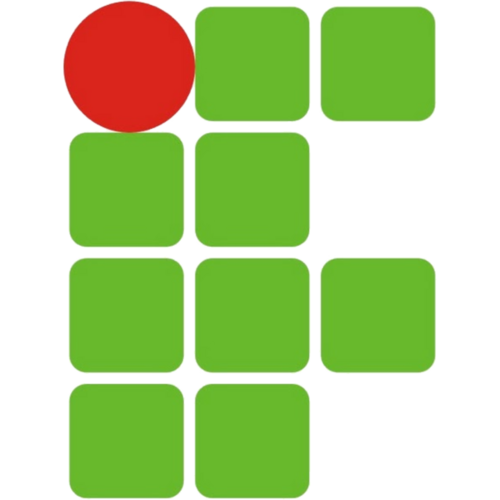
\includegraphics[scale=0.2]{img/IFRN}
	\titlepage
\end{frame}

\logo{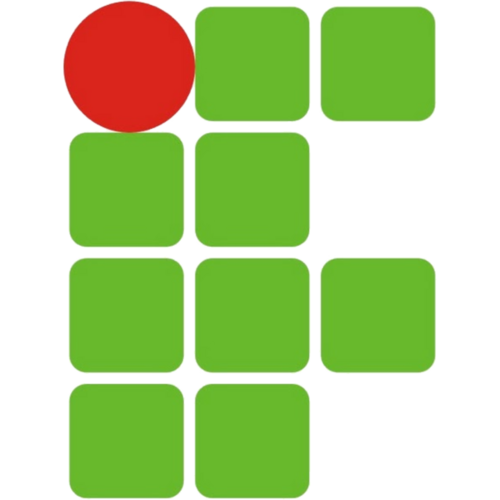
\includegraphics[scale=0.1]{img/IFRN}}

\begin{frame}
	\frametitle{O que é o Método Kanban?}

	\begin{block}{Defini\c cão}
	É um método para definir, gerenciar e melhorar serviços que fornecem o trabalho do conhecimento.
	\end{block}
\end{frame}

\begin{frame}
	\frametitle{Onde posso aplicar o método?}

	\begin{itemize}
		\item Área de TI;
		\item Agências de marketing;
		\item Recursos humanos;
		\item Servi\c cos de mídia e design;
		\item Suporte ao cliente;
		\item Desenvolvimento de produtos; e
		\item Educa\c cão.
	\end{itemize}
\end{frame}

\begin{frame}
	\frametitle{Valores}

	\begin{itemize}
		\item Transparência;
		\item Equilíbrio;
		\item Colabora\c cão;
		\item Foco no cliente;
		\item Fluxo;
		\item Lideren\c ca;
		\item Compreensão;
		\item Acordo; e
		\item Respeito.
	\end{itemize}
\end{frame}

\begin{frame}
	\frametitle{Princípios}

	\structure{Gestão da Mudança}
	
	\begin{itemize}
		\item Comece o que você tem hoje;
		\item Concorde em buscar melhorias; e
		\item Incentive atos de liderança em todos os níveis.
	\end{itemize}

	\structure{Entrega de Serviços}
	
	\begin{itemize}
		\item Compreender e focar as necessidades e expectativas dos clientes;
		\item Gerenciar o trabalho; e
		\item Evoluir políticas para melhorar os resultados.
	\end{itemize}	
\end{frame}

\begin{frame}
	\frametitle{Práticas Gerais}
	
	\begin{itemize}
		\item Visualizar;
		\item Limite do trabalho em progresso;
		\item Gerenciar o fluxo;
		\item Tornar as políticas públicas;
		\item Implementar ciclos de feedback; e
		\item Melhorar colaborativamente e evoluir
experimentalmente.
	\end{itemize}
\end{frame}

\begin{frame}
	\frametitle{Quadro}
	
	\begin{itemize}
		\item É o meio mais comum de visualizar o sistema;
		\item O trabalho é puxado da esquerda para direita;
		\item Itens de trabalho são normalmente exibidos em cartões;
		\item Os passos individuais no fluxo de trabalho são mostrados em colunas;
		\item Diferentes cores de cartões podem ser usadas para representar diferentes tipos atividades ou de grupo de clientes; e
		\item Deve refletir o seu fluxo de trabalho.
	\end{itemize}\vfill
	
	\begin{center}
		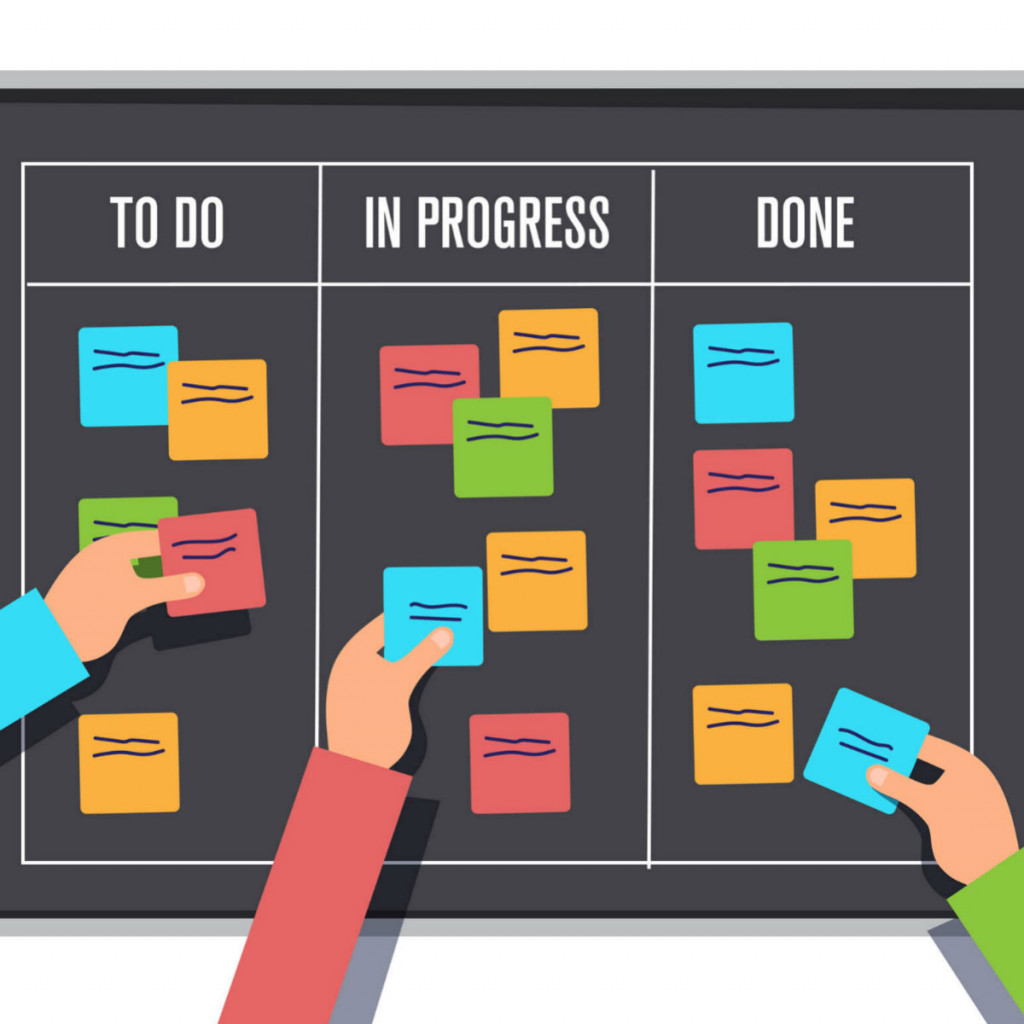
\includegraphics[scale=0.13]{img/quadro}
	\end{center}
\end{frame}

\begin{frame}
	\frametitle{Classe de Servi\c cos}
	
	\begin{itemize}
		\item Urgente;
		\item Importante;
		\item Média; ou
		\item Baixa.
	\end{itemize}
\end{frame}

\begin{frame}
	\frametitle{Métricas}
	
	\begin{itemize}
		\item Lead Time;
		\item Throughput; e
		\item WIP.
	\end{itemize}
\end{frame}

\begin{frame}
	\frametitle{Cadências}
	
	\begin{itemize}
		\item Team Kanban Meeting (Diária);
		\item Team Retrospective (Quinzenal ou mensal); e
		\item Internal Team Replenishment Meeting (Semanal ou quando
necessário).
	\end{itemize}
\end{frame}

\begin{frame}
	\frametitle{Systems Thinking Approach To Introducing Kanban (STATIK)}
	
	\begin{itemize}
		\item Identificar fontes de insatisfação;
		\item Analisar a demanda;
		\item Analisar as capacidades do sistema;
		\item Modelar o fluxo de trabalho;
		\item Identificar as classes de serviço; e
		\item Projetando o sistema Kanban.
	\end{itemize}
\end{frame}

\end{document}